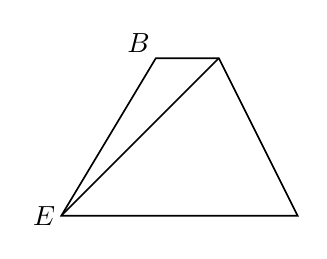
\begin{tikzpicture}[x=1cm,y=1cm,font=\normalsize,
 geometry edge/.style={solid,line width=.6pt},
 geometry mark/.style={solid,line width=.6pt},
 geometry label/.style={font=\normalsize,inner sep=2pt}]
\coordinate (B) at (1.2,2.0);
\coordinate (Q1) at (2.0,2.0);
\coordinate (Q2) at (3.0,0.0);
\coordinate (E) at (0.0,0.0);
\draw[geometry edge] (B)--(Q1)--(Q2)--(E)--cycle;
\draw[geometry edge] (E)--(Q1);
\node[geometry label,above left] at (B) {$B$};
\node[geometry label,left] at (E) {$E$};
\end{tikzpicture}